\documentclass{article}

\usepackage{minted}
\usepackage[most]{tcolorbox}
\usepackage{geometry}
\usepackage{enumitem}
\usepackage{hyperref}
\usepackage{hyperref}
\usepackage[parfill]{parskip}
\usepackage{wrapfig}
\usepackage{accsupp}

\geometry{margin=0.8in}
\definecolor{lightgreen}{rgb}{0.56, 0.93, 0.56}
\definecolor{moonstoneblue}{rgb}{0.45, 0.66, 0.76}
\definecolor{magenta}{rgb}{0.8,0.66,0.76}
\begin{document}
\BeginAccSupp{}
\begin{flushright}
Computational Biology ~\\
Tufts University Bio 35 ~\\
Fall 2021 ~\\ ~\\
\end{flushright}
\begin{center}{\textbf{\Large{Spotlight 7: Erich Jarvis}}}\end{center}

\textit{Please note that in general I have taken/adapted the words of our Spotlight subjects from their own websites to describe their work. I have done this in an effort to maintain accuracy in describing their research programs. Please do not copy paste text from their papers/websites in your assignments!}

\begin{wrapfigure}{L}{0.14\textwidth}
\begin{center}
 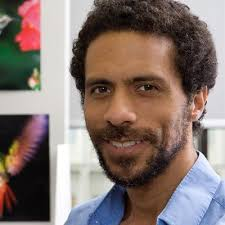
\includegraphics[width=0.13\textwidth]{images/erich-jarvis.jpeg}
 \end{center}
\end{wrapfigure}
~\\ As part of our unit on identifying orthologs, we are going to explore the work of Prof. Erich Jarvis. The Jarvis lab studies the neurobiology of vocal communication. We use vocal communication as a model behavior to know how the brain generates, perceives, and learns behavior. Emphasis is placed on the molecular pathways involved in the perception and production of learned vocalizations. We use an integrative approach that combines behavioral, anatomical, electrophysiological, and molecular biology techniques. The main animal model used is songbirds, one of the few vertebrate groups (among parrots, hummingbirds, humans, whales, dolphins and elephants) that evolved the ability to learn vocalizations. The overall goal of the research is to advance knowledge of the neural mechanisms for vocal learning and basic mechanisms of brain function. Dr. Jarvis is a faculty member at The Rockefeller University.
~\\ 

Please listen to the following radio segment (you can start around the 9:25 mark):
\begin{enumerate}
\item \texttt{\href{https://science.sciencemag.org/content/346/6215/1384.2/}{https://science.sciencemag.org/content/346/6215/1384.2}}
\end{enumerate}
And read the following article by Prof. Jarvis: 
\begin{enumerate}
\item \texttt{\href{https://science.sciencemag.org/content/sci/346/6215/1275.full.pdf}{https://science.sciencemag.org/content/sci/346/6215/1275.full.pdf}}
\end{enumerate}

\subsubsection*{Written Assignment} 
After reading about Erich Jarvis please write a reflection (max one page) on what you discovered. You might wish to address some of the following: 

\begin{enumerate}
\item What was most interesting to you in reviewing these resources?
\item What did you learn from these resources about gene duplication and the evolution of gene families? Why is it important to be able to identify orthologs to answer these questions?
\item What new questions do you have after reviewing these resources?
\item What do these resources tell you about the types of people that do computational biology, or their motivations?
\end{enumerate}

\EndAccSupp{}
\end{document}